\chapter{Laboratorio 2}
In questa esperienza di laboratorio, si sono analizzati tre circuiti che svolgono la funzione di raddrizzatori grazie alla presenza di uno o più diodi (\Fig\ref{fig:diodo}). In particolare, si è utilizzato il diodo 1N4148 \url{https://www.diodes.com/assets/Datasheets/ds12019.pdf}.
\begin{figure}[h]
	\centering
	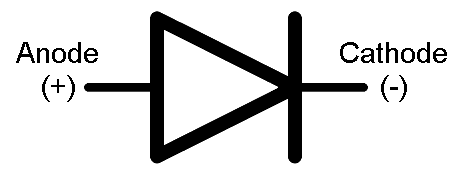
\includegraphics[width=0.3\linewidth]{./ImageFiles/Laboratorio 2/diodo_1}
	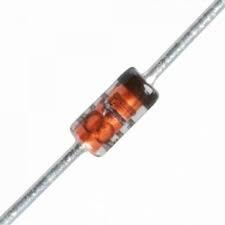
\includegraphics[width=0.2\linewidth]{./ImageFiles/Laboratorio 2/diodo_4}
	\caption{Rappresentazione simbolica di un diodo e foto del diodo 1N4148.}
	\label{fig:diodo}
\end{figure}
Il diodo è un dipolo che permette di realizzare circuiti raddrizzatori grazie al suo comportamento che differisci in base alle condizioni del circuito in cui è inserito. In particolare, se la tensione all'anodo è maggiore di una certa tensione soglia (tipicamente considerata pari a \SI{0.7}{\volt}) rispetto alla tensione a cui si trova il catodo, permette il passaggio di corrente dall'anodo al catodo. Al contrario, non è consentito il passaggio di corrente dal catodo all'anodo. Più precisamente, la relazione corrente-tensione è descritta da un a legge esponenziale:
\begin{equation}
	I_D=I_S[e^{\frac{V_D}{V_T}}-1],
\end{equation}
con I\sub{D} la corrente nel diodo (con verso positivo dall'anodo al catodo), I\sub{S} corrente inversa, V\sub{D} differenza di tensione anodo-catodo e V\sub{T} tensione termica. In figura \ref{fig:diodo_caratteristica} sono rappresentati i due modelli ideale e reale del diodo. In particolare, si definirà regione di funzionamento diretta quando il diodo è acceso e permette il passaggio di corrente da anodo a catodo ($V_{D}>0$) e regione inversa quando il diodo è spento e impedisce il passaggio di corrente (o più precisamente, avremo una corrente pari a -I\sub{S}).
\begin{figure}[h]
	\centering
	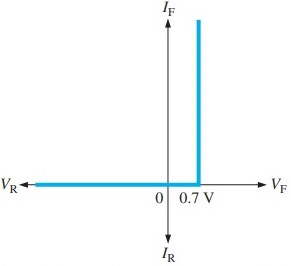
\includegraphics[width=0.3\linewidth]{./ImageFiles/Laboratorio 2/diodo_2}
	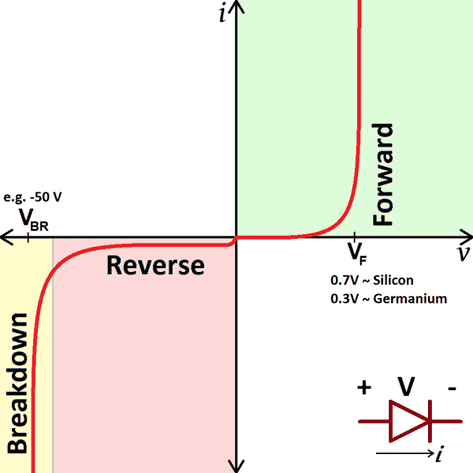
\includegraphics[width=0.3\linewidth]{./ImageFiles/Laboratorio 2/diodo_3}
	\caption{Caratteristica corrente-tensione ideale e reale di un diodo.}
	\label{fig:diodo_caratteristica}
\end{figure}

Il primo circuito realizzato è un semplice raddrizzatore a singola semionda che utilizza un singolo diodo e una resistenza. Lo schema del circuito è riportato in figura \ref{xxx}.
\begin{figure}[h]
	\centering
	%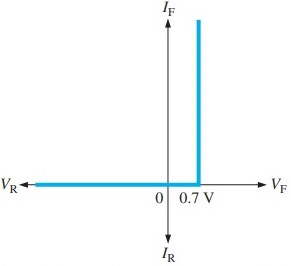
\includegraphics[width=0.3\linewidth]{./ImageFiles/Laboratorio 2/diodo_2}
	\caption{circuito}
	%\label{fig:diodo_caratteristica}
\end{figure}\todo{inserire schema e foto del circuito. indicare con D i diodi, R resistenze}
Considerando il modello ideale di diodo, è possibile analizzare il comportamento del circuito quando in ingresso è applicata una tensione sinusoidale. Considerando una tensione di soglia del diodo pari a \SI{0.7}{\volt} si ha che:
\begin{itemize}
	\item se $v_{in}>\SI{0.7}{\volt}$ allora v\sub{out}=\SI{0}{\volt}, poiché nel circuito non scorre corrente, nemmeno nella resistenza R che quindi mantiene a massa il nodo v\sub{out};
	\item se $v_{in} >= \SI{0.7}{\volt}$ il diodo D si accende; quindi sul nodo v\sub{out} avremo $v_{out}=v_{in}-\SI{0.7}{\volt}$.
\end{itemize}
Per analizzare il comportamento del circuito si sono effettuate delle misure tramite l'oscilloscopio sui nodi v\sub{in} e v\sub{out}, applicando in ingresso sul nodo v\sub{in} una sinusoide di ampiezza picco-picco di \SI{2}{\volt} e variando il valore della resistenza e della frequenza del segnale in ingresso. Nella tabella \ref{tab:valori_componenti_1} sono indicati i valori nominali e misurati delle resistenze utilizzate. \`E stata inoltre misurata la tensione di soglia del diodo utilizzato. Essa è pari a \SI{0.618}{\volt}.

\def\arraystretch{1.3}
\begin{table}[h]
	\centering
	\begin{tabular}{|c|c|c|}
		\hline
		Componente	& Valore Nominale & Valore Misurato \\ \hline
		R\sub{1}          & \SI{0}{\kilo\ohm} &     \SI{0}{\kilo\ohm}  \\ \hline
		R\sub{2}          & \SI{0}{\kilo\ohm} &     \SI{0}{\kilo\ohm} \\ \hline
		R\sub{3}          & \SI{0}{\kilo\ohm} &     \SI{0}{\kilo\ohm} \\ \hline
		R\sub{4}          & \SI{0}{\kilo\ohm} &     \SI{0}{\kilo\ohm} \\ \hline
	\end{tabular}
	\caption{Valori nominali e misurati delle resistenze utilizzate nel circuito.}
	\label{tab:valori_componenti_1}
\end{table}
Nella figura \ref{fig} sono rappresentate le differenti misure effettuate a frequenza fissa pari a xxx, variando la resistenza utilizzata.
\todo{inserire immagini R diverse e stessa frequenza}
Come si può osservare, in un diodo reale c'è una dipendenza della tensione di soglia dalla corrente che lo attraversa. Infatti, aumentando la resistenza, la tensione di soglia diminuisce. Infatti, la corrente che circola nel circuito diminuisce. Al contrario, diminuendo il valore della resistenza R, aumenta la corrente e quindi aumenta la tensione di soglia.
Successivamente si è analizzato il comportamento in frequenza del circuito, variando la frequenza della sinusoide in ingresso. Per le misure, si sono scelte le frequenze di \SI{1}{\kilo\hertz}, \SI{10}{\kilo\hertz}, \SI{100}{\kilo\hertz} e \SI{1}{\mega\hertz} \ref{fig}.
\todo{inserire immagini con frequenze diverse}
Osservando le acquisizioni si nota che aumentando la frequenza il segnale in uscita presenta una semionda distorta. In particolare, il diodo riesce a seguire abbastanza correttamente il fronte di salita del segnale in ingresso (il diodo in questa fase si accende). Tuttavia, il diodo non è sufficientemente veloce nella fase di spegnimento, producendo un onda che lentamente ritorna a zero \todo{non so come dirla meglio vediamo.}. Questo comportamento asimmetrico è presente a causa dei differenti tempi di accensione e spegnimento che caratterizzano un diodo reale. Questi tempi sono determinati dai tempi necessari alla formazione ed eliminazione della regione di svuotamento nel passaggio dalla regione diretta e inversa del diodo.  

Il circuito precedente presenta un offset significativo tra la tensione v\sub{in} e v\sub{out}. Infatti, esso è pari alla tensione di soglia del diodo che varia a seconda delle condizioni del circuito in cui il diodo è inserito. Per eliminare questo problema, si può utilizzare un diverso circuito che, utilizzando un amplificatore operazionale, consente di eliminare l'offset. Lo schema del circuito è presentato in figura xx.
\todo{inserire schema e foto circuito 2. mettere anche v1 e V-}
Per analizzare il circuito, è utile suddividere due casi:
\begin{itemize}
	\item se $v_{in}>=0$, il diodo D è acceso e il circuito si comporta come un buffer di tensione. Essendo $v_{out}=v_{in}>0$, avremo una corrente nella resistenza R che scorre verso massa. Questa corrente è fornita dall'opamp e per cui polarizza il diodo. La tensione v\sub{1} sarà invece $v_1=v_{out}+V_D=v_{out}+\SI{0.7}{\volt}$;
	\item se $v_{in}<0$, il diodo D è spento e l'amplificatore operazionale non è più retroazionato. All'interno della resistenza non scorre corrente e quindi il nodo v\sub{out} è mantenuto a una tensione di \SI{0}{\volt}. In questo caso, l'opamp si comporta come un comparatore. Per cui, essendo v\sub{in} negativa, v\sub{1} si porta alla tensione di saturazione negativa dell'amplificatore.
\end{itemize}
In questo circuito, si è mantenuto costante il valore di R, mentre si è variata la frequenza del segnale in ingresso fig xxx.
\todo{inserire foto}
\todo{inserire problema slew rate}
Analizzando più in dettaglio il comportamento del circuito, si nota un ritardo di circa \SI{4.08}{\micro\second} del fronte di salita dell'uscita rispetto all'ingresso \ref{fig}. Questo andamento è causato dal fatto che, non appena v\sub{in} diventa maggiore di zero, l'uscita deve saltare dalla tensione di saturazione negativa al valore del segnale in ingresso. Il tempo necessario all'amplificatore per effettuare questa transizione è regolato da un parametro tipico degli amplificatori operazionali definito \textit{slew rate}. \todo{da rifare e continuare------}
\todo{aggiungere figura 38}
\todo{terzo circuito}